\documentclass[a4paper]{article}
\usepackage[utf8]{inputenc}
\usepackage[warn]{mathtext}
\usepackage[russian]{babel}

\usepackage{natbib}

\usepackage{caption}
\usepackage{graphicx}
\graphicspath{}
\DeclareGraphicsExtensions{.pdf,.png,.jpg}
\DeclareSymbolFont{T2Aletters}{T2A}{cmr}{m}{it}
\usepackage{subcaption}

\usepackage{pgfplots}
\pgfplotsset{compat=1.9}

\usepackage{csvsimple}

\usepackage{subfiles}

\begin{document}
\begin{minipage}{0.8\textwidth}
\begin{center}
    \large{Санкт-Петербургский национальный исследовательский университет информационных технологий, механики и оптики
\\УЧЕБНЫЙ ЦЕНТР ОБЩЕЙ ФИЗИКИ ФТФ}
\medbreak
\end{center}
\end{minipage}
\hfill
\begin{minipage}{0.3\textwidth}

\includegraphics[scale=0.4]{itmo.jpg}
\end{minipage}

\noindent\rule{\textwidth}{1pt}
\medbreak
\begin{minipage}{0.5\textwidth}
Группа $\textit{P3112}$						
\\Студент $\textit{Сенина Мария Михайловна}$			
\\Преподаватель $\textit{Сорокина Е К}$
\end{minipage}
\hfill
\begin{minipage}{0.4\textwidth}
К работе допущен
\\Работа выполнена
\end{minipage}

\bigbreak

\begin{center}
        \Large{\textbf{Рабочий протокол и отчёт по лабораторной работе № 1.09V}}
   \LARGE{\textbf{\\Определение момента инерции методом
крутильных колебаний}}
\end{center}

\section{Цель работы}
Определение момента инерции разных тел.

\section{Задачи, решаемые при выполнении работы}
\begin{enumerate}
    \item Определение момента инерции различных твердых тел методом
крутильных колебаний.
    \item Проверка справедливости теоремы Гюйгенса-Штейнера.
\end{enumerate}

\section{Объект исслевдования}
Крутильная пружина и объектры разных масс и форм.

\section{Метод экспериментального исследования}
 
\section{Рабочие формулы}
\begin{enumerate}
    \item Среднее значение - $\frac{\sum_{i=1}^n x_i}{n}$
    \item Коэфициенты уравнения прямой через МНК $Y = aX + b$ \\ $a = \frac{n \sum_{i=1}^n (x_i - \overline{x})(y_i - \overline{y})}{\sum_{i=1}^n (x_i - \overline{x})^2}, b = \overline{y} - b\overline{x}$
    \item СКО коэффицентов уровнения прямой - $\sigma_a = \sqrt{\frac{\sum_{i=1}^n d_i}{D (n-2)}}, \sigma_b = \sqrt{(\frac{1}{n}+\frac{\overline{x}^2}{D})\frac{\sum_{i = 1}^n d^2_i}{n - 2}}$, где $d_i = y_i - (b + a x_i)$, а $D = \sum_{i=1}^n(x_i -\overline{x})^2$
    \item Погрешность измерений через коэффицент Стьюденса $\Delta x = t_{a_{дов, N}}\sqrt{\frac{\sum\limits_{i=1}^N (x - \bar{x})^2}{N (N-1)}}$, где $t_{a_{дов, N}}$ - коэффицент Стьюдентса для доверительной вероятности $a_{дов}$ и количества измерений $N$.
\end{enumerate}
\section{Измерительные приборы}
$\textbf{Погрешности измерительных приборов}$

\begin{tabular}{ l | l | l | l }\hline
№ & Наименование & Используемый диапазон & Погрешность прибора \\ \hline
1 &	Секундомер & 2,5 - 8,5 с & 	0,0001 с \\   \hline
\end{tabular}

\section{Схема установки}

\begin{figure}[h!]
   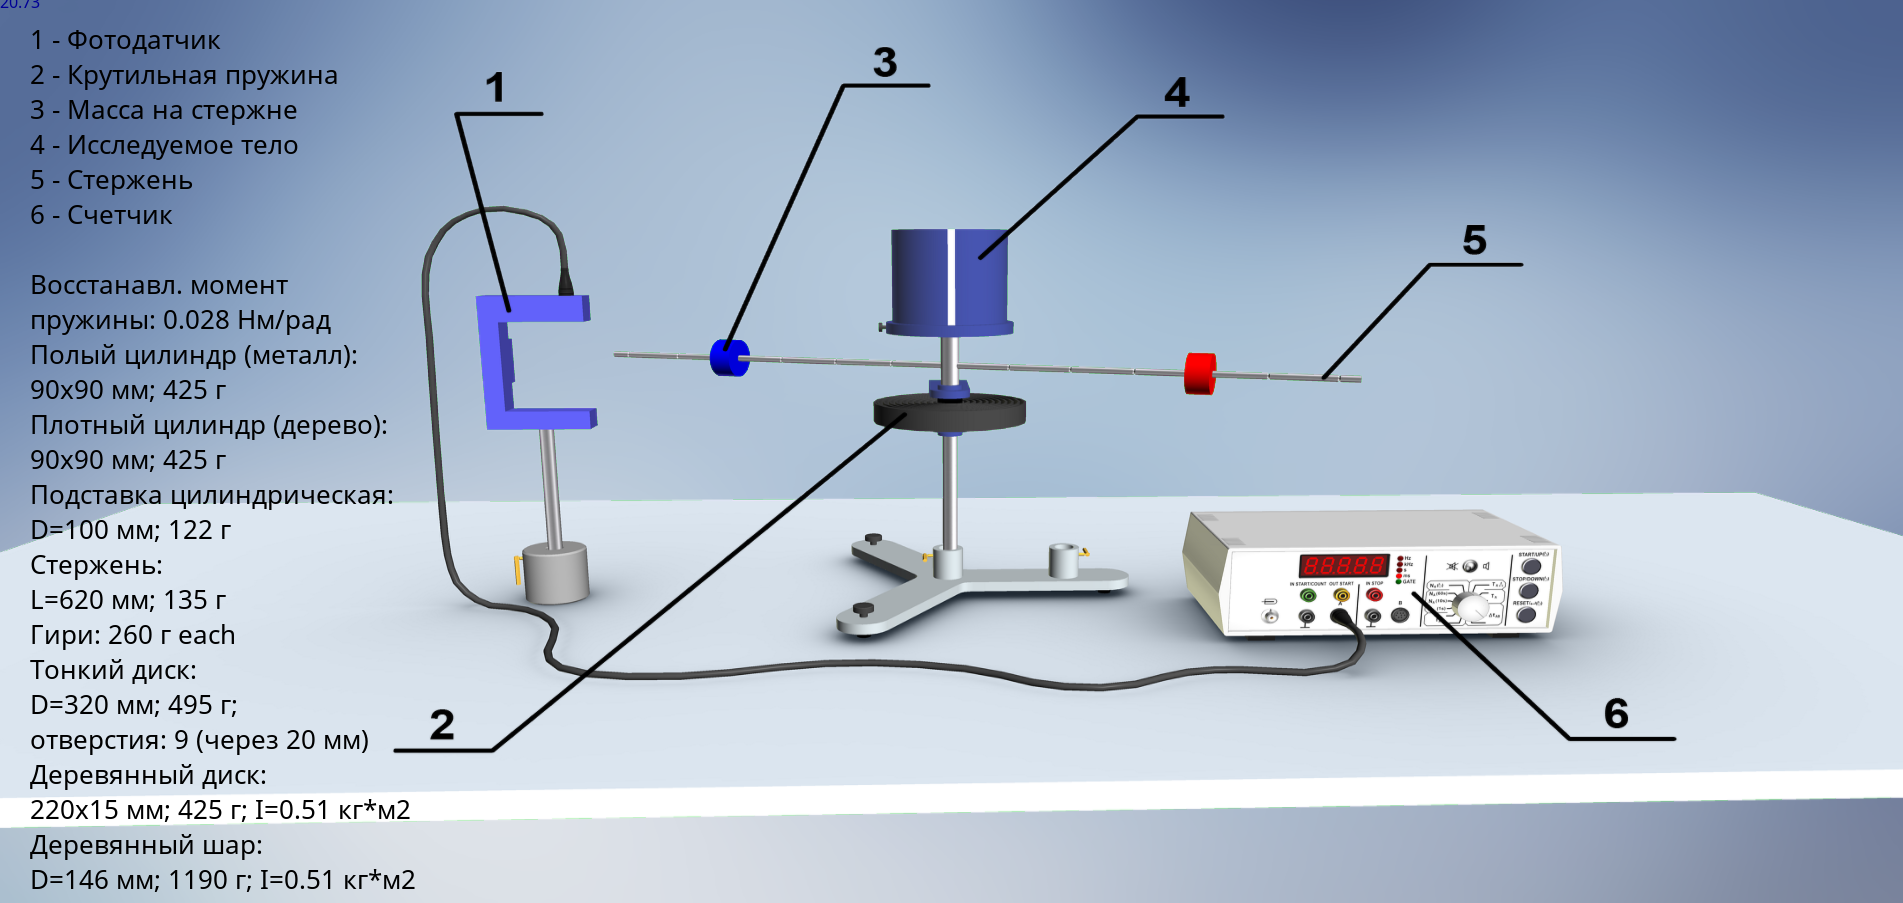
\includegraphics[scale=0.3]{stend_final.png}
    % \caption{Стенд лаборатории механики (общий вид):\\ 1 - фотодатчик, 2 - крутильная пружина, 3 - груз на стержне, 4 - объект, 5 - стержень, 6 -  хронометр.}
    \label{stend}
\end{figure}

\section{Результаты прямых измерений}
См. в приожении 1

\section{Расчёт результатов косвенных измерений}

\section{Графики}
\subfile{plot1}
\subfile{plot2}

\section{Окончательные результаты}

\section{Выводы}

\end{document}